% Nuclear Energy

\documentclass[11pt]{article}

\usepackage[a4paper, margin=1in]{geometry}

\usepackage{amsmath}

\usepackage{amssymb}

\usepackage[german]{babel}

\usepackage[autostyle=true]{csquotes}

\usepackage{libertine}

\usepackage[libertine]{newtxmath}

\usepackage{tikz}

\usepackage{gensymb}

\usepackage{fancyhdr}

\usepackage{amsfonts}

\usepackage{pgfplots}

\pgfplotsset{compat=1.10}

\usepackage{multicol}

\usepackage{caption}

\usepackage{floatrow}

\everymath{\displaystyle}

% Header / footer settings

\pagestyle{fancy}
\fancyhf{}
\renewcommand{\headrulewidth}{0.2mm}
\fancyhead[C]{Funktionen}
\renewcommand{\footrulewidth}{0.2mm}
\fancyfoot[L]{Peter Goldsborough}
\fancyfoot[C]{\thepage}
\fancyfoot[R]{\today}

\fancypagestyle{plain}{%
	\fancyhf{}
	\renewcommand{\headrulewidth}{0mm}%
	\renewcommand{\footrulewidth}{0.2mm}%
	\fancyfoot[L]{Peter Goldsborough}
	\fancyfoot[C]{\thepage}
	\fancyfoot[R]{\today}
}


\setlength{\headheight}{15pt}

\setlength{\parindent}{0pt}

\addtolength{\parskip}{\baselineskip}


\newcommand{\overbar}[1]{\mkern 1.5mu\overline{\mkern-1.5mu#1\mkern-1.5mu}\mkern 1.5mu}

\newcommand{\heading}[1]{\begin{center}\Huge \textbf{#1}\end{center}\par}

\newcommand{\sub}[1]{\vspace{\parskip}{\LARGE\textbf{#1}}}

\newcommand{\subsub}[1]{{\Large \textbf{#1}}}

\newcommand{\subsubsub}[1]{\textbf{#1}}

\newcommand{\colvec}[1]{\begin{pmatrix}#1\end{pmatrix}}

\newcommand{\extrapar}{\par\vspace{\baselineskip}}

\newcommand{\zitat}[1]{\foreignquote{german}{#1}}

\newcommand{\bolditem}[1]{\item \textbf{#1}}

\newcommand{\titleitem}[1]{\bolditem{#1}\par}

\newcommand{\defas}{ \dots \,\,}

\begin{document}
\thispagestyle{plain}

\heading{Nuclear Energy}

\sub{The Atomic Nucleus}

The nucleus of an atom is found at its core and is surrounded by electrons, who, in turn, are found in orbitals --- regions of high probability --- in one of several fixed (\emph{quantized}) energy states. The atomic nucleus as we know it is made up of two types of subatomic particles: \emph{protons} and \emph{neutrons}. Protons, denoted either by $p$, $p^+$ or $\ce{^1_1p}$ (in \emph{isotope notation}), are positively charged particles whose charge is equal to the positive elementary charge, i.e. $+1$ and whose mass is slightly less than that of a neutron but approximately 2000 times greater than that of an electron. On the other hand, a neutron, denoted by $n$, $n^0$ or $\ce{^1_0n}$, carries no charge. Collectively, neutrons and protons are referred to as \emph{nucleons}, as they make up the nucleus of an atom. Both neutrons and protons have a mass approximately equal to one \emph{atomic mass unit} (amu), whose conversion factor to kilograms is about $1.66 \cdot 10^{-27}$ kg per amu. Nucleons numbers of an atom can be determined from its isotope notation, which is of the general form: $$\ce{^A_ZX}$$ Here, $Z$ is the proton number and is commonly given the name \emph{atomic number}, as the number of protons determines the element $X$ of an atom. $A$ is the number of nucleons, i.e. the sum of protons and neutrons of the atom. To determine how many neutrons an atom has, one would thus deduct $Z$ from $A$. $A$ is referred to as the \emph{mass number} of the atom, as $A$ is equivalent to how many atomic mass units the atom weighs (approximately). An element may have many \emph{isotopes}, all of which have the same number of protons, i.e. atomic number $Z$, while they differ in the number of neutrons and thus in their mass number $A$. For example, Carbon-11 (notice $11$ denotes the isotope in this spoken notation) $\ce{^{11}_6C}$ is one isotope of the Carbon element with 5 neutrons (11 nucleons), while Carbon-14 $\ce{^{14}_6C}$ (used for archelogical dating of organic matter) is another isotope of Carbon with 8 neutrons. The different isotopes of an atom share chemical properties, but may differ greatly in nuclear stability, i.e. one may be radioactive while another may be stable.

\subsub{The Strong Nuclear Force}

One of the two types of subatomic particles found in the nucleus, i.e. one of the two types of \emph{nucleons}, has a positive electrical charge: protons. These are found very close together in the nucleus. However, according to the laws that govern how electrically charged particles interact, like charges, i.e. protons and protons, should repell. There must obviously be some force that counteracts the electrostatic force of repulsion between protons, else a nucleus could never form. This force is called the \emph{strong nuclear force} and is the attractive force acting between nucleons. It has a very short range of only about one femtometer ($10^{-15}$ m) but is, as its name implies, very strong --- about 100 times stronger than the gravitational force. The strong nuclear force acts only inside the nucleus, only on nucleons and not on electrons. Moreover, the effectiveness of the strong nuclear force determines the stability of an atom. When an atom has an imbalanced neutron-to-proton ratio or is simply too heavy, the strong nuclear force is too weak to hold all nucleons inside the nucleus together. Such an unstable atom is then referred to as being \emph{radioactive} --- it will emit radiation either in form of an $\alpha$ or $\beta$ particle or a $\gamma$ photon.

\subsub{Binding Energy and Mass Defect}

When an object is at rest on the surface of the earth at sea level, it it said to have no \emph{gravitational potential energy}. When the object is lifted to a certain height, work must be done against the attraction the gravitational force exerts between the object and earth. Once at a certain height $h$, the object stores gravitational potential energy equivalent to $m \cdot g \cdot h$ where $m$ is its mass and $g$ the acceleration of gravity. A similar argument applies to nucleons in the nucleus of an atom. The strong nuclear force, albeit a short-ranged force, exerts an enormous attractive pull on protons to counteract their mutual electrostatic repulsion. To overcome this force, work must be done against it, similar to how energy must be invested to lift an object to a certain height. This amount of work done against the strong nuclear force is referred to as the \emph{binding energy} of the nucleus and defined as:

\begin{displayquote}

	The energy that must be invested to split or break a nucleus into its constituent, separate, non-interacting nucleons.

\end{displayquote}

Once an object is lifted to a certain height in a gravitational field, it stores gravitational potential energy, i.e. energy by virtue of its \emph{position}. Once more, this is similar to how nucleons, once separated, store energy as a result of their position. Interestingly, this energy is contained in the mass of the protons and neutrons according to Einstein's mass-energy equivalence $E=mc^2$. Thus, the constituent, non-interacting, \emph{free} nucleons have a greater mass than when bound by the strong nuclear force in the nucleus of an atom. Were the constituent, free nucleons to be bound back together to form a nucleus once more, they would lose the energy stored in their mass just like a falling object loses gravitational potential energy. Thus, the second definition of binding energy, more suitable to its name, reads:

\begin{displayquote}
	
	The energy released when binding free nucleons to a nucleus.

\end{displayquote}

Thus, to recapitulate, binding energy is the energy that must be supplied to work against the strong nuclear force and break a nucleus into its consituent protons and neutrons, and is the energy set free when binding those nucleons back to a nucleus to be kept in place by the strong nuclear force. The amount of binding energy that needs to be invested for a certain nucleus can be calculated from its \emph{mass defect}. The mass defect $\Delta m$ is the difference between the sum of masses of the heavier, free nucleons and the sum of masses of the nucleons of the atom once bound, i.e. the mass of the nucleus. This value can be calculated by multiplying the proton or atomic number $Z$ of an atom by the proton mass $m_p$, adding to that the product of the neutron number $A - Z$ and the neutron mass $m_n$, and deducting from this sum the mass of the nucleus $m_{nucleus}$: $$\Delta m = Z \cdot m_p + (A - Z) \cdot m_n - m_{nucleus}$$ The binding energy $E$ may then be found according to the mass-energy relation $E = mc^2$. As an example, consider a uranium-238 nucleus: $\ce{^238_92U}$. One would first calculate the sum of masses of its constituent nucleons (92 protons and $238 - 92 = 146$ neutrons): $$92 \cdot m_p + (238 - 92) \cdot m_n = 92 \cdot 1.67262 \cdot 10^{-27} + 146 \cdot 1.67493 \cdot 10^{−27} = 3.98420 \cdot 10^{25} kg$$ Then, it can be found that the mass of a uranium-238 nucleus is approximately $3.95292 \cdot 10^{-25}$ kg. The mass defect $\Delta m$ would thus be equal to: $$\Delta m = m_{nucleons} - m_{nucleus} = 3.12822 \cdot 10^{-27}\, kg$$ To now calculate the binding energy, i.e. the difference energy the costituent, free, non-interacting nucleons store in their mass and that is released when re-bound, one uses the Einstein mass-energy equivalence formula: $$E = m \cdot c^2 = 3.12822 \cdot 10^{-27} \cdot (3 \cdot 10^8)^2 = 2.81540 \cdot 10^{-10} J$$ This value is now in the SI-unit Joules and is thus a very small value. More commonly, one would convert this to electron-volts $[eV]$. One Joule is equal to $6.241509 \cdot 10^18$ eV, thus the total binding energy of the uranium nucleus is: $$E = 2.81540 \cdot 10^{-10} \cdot 6.24151 \cdot 10^18 = 1.75771 \cdot 10^{9}\, eV \approx 1758\, MeV$$ A more useful measure of the stability of a nucleus is given by its \emph{binding energy per nucleon} rather than its total binding energy. It is calculated simply by dividing the total binding energy $E$ required to split up a nucleus by its number of nucleons $A$: $$\text{BEPN } = \frac{E}{A}$$ For the uranium isotope with 238 nucleons given before this value would equal: $$\frac{1.75771 \cdot 10^{9}}{238} = 7.38273 \text{ MeV per nucleon}$$
Hydrogen and Helium isotopes, the lightest nuclei, have low BEPN values, while heavier nuclei such as Uranium or Plutonium typically have binding-energy-per-nucleon values in the range of 7 to 9 MeV per nucleon. Hydrogen-1 consists only of a proton, thus it has no binding energy, as is it not bound to any other nucleons. Also, it should be said that the most stable nucleus of all is iron-56, i.e. it requires the most binding-energy-per-nucleon to be invested to split it into its constituent nucleons. This is important as it will be seen that for both fission and fusion iron is the threshold after which energy is no longer released but needs to be invested for the reaction to occur. Below is an approximate representation of the binding energy per nucleon and nucleon number relationship for nuclei.

\begin{plot}
	
	% BEPN axis
	\draw (0, 0) -- ++(0, 5) node [above] {BEPN [MeV/nucleon]};

	% BEPN ticks
	\foreach \y in {0, 1, ..., 9}
	{
		\draw (0, {\y/2 + 0.01}) node {$-$};

		\draw (-0.3, {\y/2}) node {\y};
	}

	% Nucleon number axis
	\draw (0, 0) -- ++(9.5, 0) node [right] {Nucleons $A$};

	% Nucleon number ticks
	\foreach \x in {30, 60, ..., 270}
	{
		\draw ({\x/30}, 0) node {$|$};

		\draw ({\x/30}, -0.5) node {\x};
	}

	% Graph
	\draw (0, 0) .. controls (0.5, 5.8) and (0.8, 4.5) .. (9, 4);

	% Iron
	\draw [<-] (1.9, 4.5) -- ++(0.5, 0.5) node [right] {Iron-56};

	% Hydrogen 1
	\draw [<-] (0.1, 0.1) -- ++(0.5, 0.5) node [right] {Hydrogen-1};

	% Helium-3
	\draw [<-] (0.2, 1.45) -- ++(0.5, 0.5) node [right] {Helium-3};

	% Uranium-238
	\draw [<-] (8.9, 3.9) -- ++(-0.5, -0.5) node [below] {Uranium-238};

	% Uranium-235
	\draw [<-] (8.7, 4.1) -- ++(-0.5, 0.5) node [above] {Uranium-235};


\end{plot}

What should be emphasized here once more is that binding energy (per nucleon) is really a measure of the stability of the nucleus. When it has a higher BEPN value, it requires more energy to be invested to split it up, i.e. it is more stable. On the other hand, isotopes of lower BEPN value, such as Uranium-238 on the far right, require less energy to be split up into their constituent, free nucleons. As such, there is certainly a relationship between the binding energy of a nucleus and the potential energy of its nucleons. The more binding energy, the more energy is required to split up a nucleus, the more stable it is, the less is its potential to undergo radioactive decay and thus the less (potential) energy the nucleons have. If, however, a nucleus has low binding energy, then it is easily broken apart and is thus less stable. Its nucleons can be thought to have lower potential energy.

This discussion sets the stage for further investigation of the two forms of nuclear reactions: \emph{nuclear fission} and \emph{nuclear fusion}. They will be thoroughly looked into in further sections of this paper, but first the basics of how binding energy makes them possible should be examined. In general, there are two conditions for the \emph{release} of energy during a nuclear reaction to take place:

\begin{enumerate}
	
	\item The mass defect $\Delta m$ between the sum of all masses of the 
	\emph{reactancts} of the nuclear reaction and the sum of all masses of the 
	\emph{products} must be \textbf{positive}.

	\item The binding energy (per nucleon) must increase, i.e. the products must be more stable than the reactants. This is achieved via a release of (potential) energy that is measured as the mass defect.

\end{enumerate}

Now it should be considered what nuclear fission and fusion are and whether the conditions set for a release of energy are obeyed, and for what (range of) nuclei:

\begin{itemize}
	
	\titleitem{Nuclear Fusion}

	Nuclear fusion is the joining or \emph{fusion} of lighter nuclei to heavier nuclei. One can observe that for binding energy values less than that of iron, fusing of lighter elements to higher elements constitutes an increase in binding energy --- the resultant, heavier nucleus is more stable than the reactants (the lighter nuclei). This means that the masses of the lighter nuclei, together, are greater than the mass of the heavier nucleus. There was thus a mass defect and energy was releaesd. On the other hand, after iron, fusion to a heavier element decreases the binding energy. This means that less energy would have to be invested to split up the resultant nucleus into its constituent nucleons than was the case for the lighter nuclei. In turn, this would indicate that the product is less stable and has more potential energy than the reactants. Where would this extra energy come from? It would have to be invested. Energy is therefore only released for nuclei with less nucleons than iron in the case of fusion.

	\titleitem{Nuclear Fission}

	Nuclear fission is the phenomenon whereby a heavier nucleus splits into two lighter, \emph{daughter nuclei}. Now, studying the BEPN table, one finds that this can only result in a positive mass defect and an increase in binding energy and stability for nucleon numbers higher than iron. In that case, the daughter nuclei are more stable than the mother nucleus, i.e. binding energy has increased, there was a positive mass defect and energy was released. For elements with less nucleons than iron, fission would result in the daughter nuclei being less stable and having less binding energy. A negative difference in binding energy $E$ between the products and the reactant would indicate a negative mass defect, meaning the daughter nuclei are heavier than the mother nucleus. If their weight was increased, their energy has increased. This energy would now have to be \emph{invested} rather than it being released. Thus, also for fusion the limit of energy release is iron. Only from uranium-238 up to iron-56 will fission result in a positive mass defect and an increase in binding energy.

\end{itemize}

One last interesting fact to mention is that when observing the BEPN graph, it can be noticed that one single nuclear fusion, e.g. from two hydrogen atoms to one helium atom, results in a much greater increase in binding energy \emph{per nucleon} and release of nuclear energy \emph{per nucleon} than a single fission reaction, e.g. from uranium-238 to uranium-235. Fusion usually results in a release of about 3-4 MeV of energy while fission reactions cause about 1 MeV of energy to be released. However, the elements involved in nuclear fusion contain fewer nucleons than fissionable nuclei. Thus, fusion reactions release more energy \emph{per kilogram} of nuclei (more fit into a kilogram) while fission reactions produce more energy \emph{per atom}.

\sub{Nuclear Fission}

Nuclear fission occurs when a heavier nucleus (heavier than iron for a release of energy) splits into two lighter daughter nuclei. Most commonly fission is brought about or by ejecting a low-energy \emph{thermal} neutron at an element known to undergo nuclear fission. This is known as \emph{induced fission}. If a nucleus simply splits into two, this is referred to as \emph{spontaneous fission}. In a nuclear fission reactor, uranium-235 is a common choice for induced fission, as it is one of the heaviest elements and is (still) quite abundant on earth. This isotope is readily fissionable, especially when the aforementioned slow, thermal neutrons are used to induce fission. However, 99.3\% of uranium ore contains an isotope of uranium with 238 nucleons, which has the problematic property of absorbing neutrons rather than letting them induce fission. As a result, uranium ore must usually be \emph{enriched}, i.e. the amount of uranium-235 is artificially increased, to ensure that the \emph{critical mass} is met --- the minimum fissionable amount of uranium. This critical mass is usually around 50 kg. There are two further noteworthy properties of uranium or fission in general that should be mentioned. The first is that there is no single way that a uranium nucleus can split when undergoing nuclear fission. There are many pairs of daughter nuclei possible, each with a different likelyhood and probability to occur, as shown in the graph below.

\begin{figure}[h!]
	\centering
	\begin{tikzpicture}
		% Grid
		\draw [help lines] (0, 0) grid (10.5, 6);
		
		% Probability axis
		\draw [thick, ->] (0, 0) -- ++(0, 6.2) node [above] {\% of Fissions};

		% Probability ticks
		\foreach \i/\l in {1/0.001, 2/0.01, 3/0.1, 4/1.0, 5/10.0}
		{
			% Tick
			\draw (0, {\i + 0.01}) node {$-$};

			% Label
			\draw (-0.5, \i) node {\l};
		}

		% Nucleon number axis
		\draw [thick, ->] (0, 0)-- ++(10.5, 0) node [right] {Nucleons $A$};

		% Nucleon number ticks
		\foreach \i in {70, 80, ..., 170}
		{
			\draw ({\i/10-7}, 0) node {$|$};

			\draw ({\i/10-7}, -0.5) node {\i};
		}

		% Curve, left part
		\draw [red] (0.2, 0) .. controls (1, 3) and (3, 5) .. (3, 4.7);
		\draw [red] (3, 4.75) .. controls (4, 5) and (4.2, 2.5) .. (5, 2);

		% Curve, right part
		\draw [red] (7, 4.75) .. controls (6, 4) and (6.2, 2.5) .. (5, 2);
		\draw [red] (9.8, 0) .. controls (9, 3) and (8, 5) .. (7, 4.75);
	\end{tikzpicture}
	\caption*{This should be symmetric}
\end{figure}

Often, the mass of the mother nucleus will split in a proportion of 40\% to 60\%. For uranium-235 with atomic number 92, this \emph{could} mean one daughter nucleus gets 36 protons and 90 nucleons in total (Krypton-90), while the other receives 56 protons and 144 nucleons in total (Barium-144). If one counts correctly, one notices that while charge of the nuclei just mentioned is conserved, the other quantity that must stay the same, the number of nucleons, did not. 90 plus 144 equal 234 and not the original 235 nucleons of the uranium mother nucleus. This introduces the second property of nuclear fission: between one and three \emph{fast, high energy neutrons} are set free during the fission reaction. This means that alongside the original thermal neutron that induced the fission, one to two further neutron will be emitted during the reaction, alongside the huge amount of energy that can be used for other purposes, such as generating energy.

Let us examine one possible nuclear fission reaction for uranium-235. A low, energy, thermal neutron will be fired towards it to induce fission. For a very short time, around $10^{-12}$ seconds (one picosecond), the nucleus will then exist as uranium-236. This is a highly unstable, excited isotope which undergoes fission very quickly. As it does so, it breaks up into two daughter nuclei of intermediate mass. The neutron shot at the nucleus is released again, alongside one to two more neutrons. These are fast and highly energetic. Also, energy will be released. This entire process is given by the following equation: $$\ce{^{235}_{92}U} + \ce{^1_0n} \rightarrow \ce{^{144}_{56}Ba} + \ce{^{90}_{36}Kr} + 2\, \ce{^1_0n} + 179 \text{ MeV of energy}$$ The energy released can be calculated by one of two ways: either via the mass defect $\Delta m$, which can be converted into energy via $E=mc^2$, or via the difference in binding energy between the daughter nuclei and the mother nucleus, as this must have increased for energy to be released.

\begin{enumerate}
	
	\titleitem{Mass Defect}

	The first method of calculating the energy released is to determine the mass defect $\Delta m$ of the reaction. This is the difference in mass between the mother nucleus and all of the products of the reaction: the two daughter nuclei plus the neutrons released --- in this case two. The atomic mass of uranium-235 is precisely 235.043929918 atomic mass units. That of Barium-144 is 143.922952853 amu, that of Krypton-90 is 89.919516555 amu and neutrons have a mass of 1.008664916 amu (not precisely one). The mass defect in atomic mass units is thus: $$m_{reactants} = 235.043929918 + 1.008664916$$ $$m_{products} = 143.922952853 + 89.91951655 + 2 \cdot 1.008664916$$ $$\Delta m = m_{reactants} - m_{products} = 0.192795599\, amu$$ This mass defect can now be converted into kg ($1, amu \approx 1.661 \cdot 10^{-27}$) and then be plugged into the mass-energy equivalence formula: $$E = m \cdot c^2 = (0.192795599 \cdot 1.661 \cdot 10^{-27}) \cdot (3 \cdot 10^8)^2 = 2.882101409 \cdot 10^{-11}\, J$$ The conversion factor between Joules and electron-volts is then $6.241509 \cdot 10^{18}$: $$E = 2.882101409 \cdot 10^{-11} \cdot 6.241509 \cdot 10^{18} = 1.798866189 \cdot 10^8\, eV = 179.8866189\, MeV$$

	\titleitem{Binding Energy}

	The second possibility to determine the energy released is to directly use the increase in binding energy between the less stable reactants and the more stable products. To do so, one uses the binding energy per nucleon values for the nuclei, multiplies them by the respective number of nucleons and determines the increase in total binding energy, which is equivalent to the energy released. The binding energy per nucleon for uranium-235 is $7.590907\, MeV\, nucleon^-1$, that of barium-144 $8.265467\, MeV\, nucleon^-1$ and that of krypton-36 $8.591377\, MeV\, nucleon^-1$. The difference in binding energy is thus: $$E = (8.265467 \cdot 144 + 8.591377 \cdot 36) - 7.590907 \cdot 235 = 179.588033\, MeV$$ This is obviously a much faster method of calculation.

\end{enumerate}

A nuclear reaction will set free between one and three fast neutrons. If further uranium nuclei are within their reach, i.e. if the aforementioned \emph{critical mass} (50kg) is available, these neutrons can induce further fission given they are \emph{slowed down}. If they are not slowed down, it is more likely that they are absorbed by uranium-238 than lead to fission of uranium-235. The process of fission inducing the fission of one or more other nuclei is referred to as a \emph{chain reaction}. We then speak of a certain multiplication factor $k$. If $k$ is equal to one, then one fission will induce exactly one more fission. Thus, the number of neutrons and fission reactions is maintained constant. This is required for a nuclear reactor to prevent overheating. If $k$ is however greater than 1, then one fission will indcue more than one fission. The number of neutrons would thus increase rapidly. This is unwanted and cause major catastrophes for nuclear reactors, but is the wanted result in case of a nuclear weapon. Lastly, $k$ may also be less than 1, in which case the number of neutrons and fissions induced gradually nears reduces and eventually stops. This may be necessary to remove the nuclides.

\subsub{Nuclear Fission Reactor}

A nuclear power station is essentially a thermal power station that converts thermal energy generated by nuclear fission reactions into mechanical energy to turn a turbine, which then powers a generator of electricity. A diagram of a nuclear generator is given below. We hear speak of a pressurized-water reactor.

\begin{figure}[h!]
	\centering
	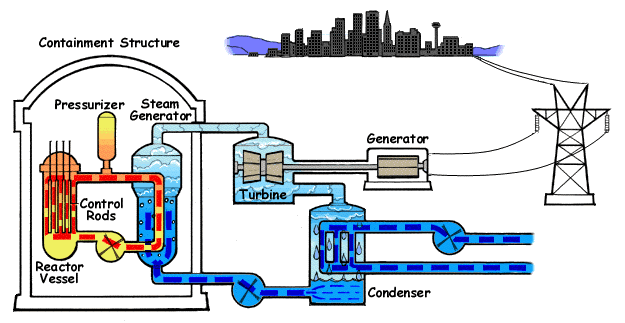
\includegraphics[scale=0.65]{img/reactor}
\end{figure}

The major components of a nuclear reactor include:

\begin{itemize}
	
	\bolditem{Fuel rods} which contain pellets of enriched uranium, consisting of 2-4\% of uranium-235 (natural uranium contains 0.7\% uranium-238). The rest is uranium-238. Neutrons hits these rods to induce fission of a nucleus inside.

	\bolditem{Control rods} commonly made of cadmium or boron, as these materials have a high probability to absorb neutrons. They are used to control the multiplication factor $k$ and especially to ensure that it stays close or equal to $1$, as a higher $k$-factor would result in too too much energy and heat being generated (which would be noticed due to the heat). This could then potentially lead to a \emph{meltdown}. The rods can be moved into or out of the reactor core to decrease or increase the power output, respectively. Also, one may want to shut down the reactions going on entirely, in which case one would move the rods into the reactor completely, for a long enough time.

	\item A \textbf{moderator}, often water, to slow down the fast neutrons ejected in the process of fission, as fast neutrons are more likely to be absorbed by U-238 rather than induce fission of U-235. Neutrons collide with water molecules and thus continuously lose momentum and speed, eventually becoming \emph{thermal} neutrons, ideal for induced fission.

	\item A \textbf{coolant}, again most commonly water (can absorb heat well), circulating within the primary water cycle of the reactor. In fact, it has two purposes. First of all, it is pumped through the reactor core to absorb the thermal energy emitted by the fission reaction and to conduct it away from the core. It then moves to the heat exchanger, where it transfers the thermal energy to the water in the secondary cycle, causing it to boil, turn into steam and then drive the turbine (which then turns a generator). In the primary water cycle, a pressurizer ensures that the coolant heated in the core does not boil (it should only do so in the secondary cycle). In the secondary cycle, a condenser then turns the steam that turned the engine back into liquid water.

	\item A \textbf{gas turbine and generator}, via which the thermal energy generated via fission reactions is turned into rotational kinetic energy and finally to electric energy to be supplied to cities.

	\item \textbf{Containment and shielding} to prevent radiation ($\gamma$) and neutrons from escaping from the reactor core. Of course, also the reactor must be protected, thus the shielding also prevents external factors from influencing the happening in the steel pressure vessel.

\end{itemize}

Many people are concerned about fission reactors. What are advantages, what are disadvantages?

\begin{itemize}

	\bolditem{Advantages:}

	\begin{itemize}

		\item Large amounts of energy produced with little input
		\item No burning of fossil fuels or greenhouse gases

	\end{itemize}

	\bolditem{Disadvantages:}

	\begin{itemize}

		\item Waste products are very dangerous, highly radioactive and cannot easily be gotten rid of.

		\item Not sustainable, uranium is a natural resource that will deplete in the next 30 to 60 years.

		\item Very dangerous, such that if an accident happen, it can cause severe damage to humans and the surrounding environment.

	\end{itemize}

\end{itemize}

\sub{Nuclear Fusion}

Nuclear fusion is the source of energy of all stars. Thus it must produce a rather large amount of energy, no? The process of fusion involves two light nuclei coming together close enough under conditions of high temperature and pressure such that the strong nuclear force may overcome the electrostatic repulsion between the protons of the nuclei and cause them to join. As always for a nuclear reaction, there must be a positive mass defect and an increas in binding energy in order for energy to be released rather than needing to be invested. Only elements lighter (with less nucleons) than iron can fuse to heavier nuclei with an increase in binding energy. After iron, fusion would result in a decrease in binding energy, i.e. a negative mass defect, meaning a positive increase in mass of the products, which in turn indicates an input of energy rather than the wanted output. One example of a fusion reaction is the joning of two deuterium atoms (hydrogen-2) to helium-4: $$\ce{^2_1H} + \ce{^2_1H} \rightarrow \ce{^4_2He} + \gamma$$ The energy is released, as can be seen, via a $\gamma$ ray photon. One important fact to mention about fusion is that it requires a certain \emph{activation energy}. This means a high enough pressure to ensure a high nuclei density (high probability for collision) and conditions of high temperatures, typically $10^8$ Kelvin, to give the nuclei sufficient speeds to collide (kinetic energy in the keV region). This is to ensure that the electrostatic force of repulsion can be overcome. 

Nuclear fusion is not yet practically implemented in the way nuclear fission is. However, it has been used for creating bombs (of course). Such a bomb is termed an H-Bomb, short for Hydrogen-Bomb. The energy in such a bomb, much greater than that of an atom bomb relying on nuclear fission (with the multiplication factor $k > 1$), is generated via fusion of hydrogen nuclei to a heavier element: helium. This is also what occurs at the core of the sun. Of course, in the future, one would like nuclear fusion to be used for the generation of energy in a power station. This would haveseveral advantages:

\begin{itemize}
	
	\item Hydrogen and other elements involved in fusion reactions (often lithium) are readily available, in fact virtually inexhaustible.

	\item None of the toxic or radioactive waste products created by nuclear fission reactors are produced. There are some waste products, of course, mainly irradiated materials that have absorbed neutrons, however they pose much less of a problem than the nuclear waste of a fission reactor.

	\item Greater energy yield per kilogram of energy produced. The reason for this is that nuclear fusion results in a higher amount of energy releasd and a higher increase in binding energy per nucleon compared to a fission reaction. It is just that hydrogen or helium contain (a lot) fewer nucleons than, say, uranium-235. However, per kilogram (into which you can fit more lighter nuclei), fusion yields more energy. It is just per atom which fission is more effective.

\end{itemize}

\subsub{Fusion Power Station}



\end{document}